\documentclass[a4paper, 12pt]{article}

\usepackage{listings}
\usepackage{indentfirst}
\usepackage{graphicx}
\usepackage{pdfpages}

\usepackage{color}

\definecolor{mygreen}{rgb}{0,0.6,0}
\definecolor{mygray}{rgb}{0.5,0.5,0.5}
\definecolor{mymauve}{rgb}{0.58,0,0.82}

\lstset{ 
  backgroundcolor=\color{white},   % choose the background color; you must add \usepackage{color} or \usepackage{xcolor}; should come as last argument
  basicstyle=\footnotesize,        % the size of the fonts that are used for the code
  breakatwhitespace=false,         % sets if automatic breaks should only happen at whitespace
  breaklines=true,                 % sets automatic line breaking
  captionpos=b,                    % sets the caption-position to bottom
  commentstyle=\color{mygreen},    % comment style
  deletekeywords={...},            % if you want to delete keywords from the given language
  escapeinside={\%*}{*)},          % if you want to add LaTeX within your code
  extendedchars=true,              % lets you use non-ASCII characters; for 8-bits encodings only, does not work with UTF-8
  keepspaces=true,                 % keeps spaces in text, useful for keeping indentation of code (possibly needs columns=flexible)
  keywordstyle=\color{blue},       % keyword style
  language=Octave,                 % the language of the code
  morekeywords={*,...},            % if you want to add more keywords to the set
  numbers=left,                    % where to put the line-numbers; possible values are (none, left, right)
  numbersep=5pt,                   % how far the line-numbers are from the code
  numberstyle=\tiny\color{mygray}, % the style that is used for the line-numbers
  rulecolor=\color{black},         % if not set, the frame-color may be changed on line-breaks within not-black text (e.g. comments (green here))
  showspaces=false,                % show spaces everywhere adding particular underscores; it overrides 'showstringspaces'
  showstringspaces=false,          % underline spaces within strings only
  showtabs=false,                  % show tabs within strings adding particular underscores
  stepnumber=2,                    % the step between two line-numbers. If it's 1, each line will be numbered
  stringstyle=\color{mymauve},     % string literal style
  tabsize=2,	                   % sets default tabsize to 2 spaces
  title=\lstname                   % show the filename of files included with \lstinputlisting; also try caption instead of title
}

%===========================================%
%=               Credits                   =%

\author{Name}
\title{Title}

%=                                         =%
%===========================================%

%===========================================%
%=               BEGIN                     =%

\begin{document}
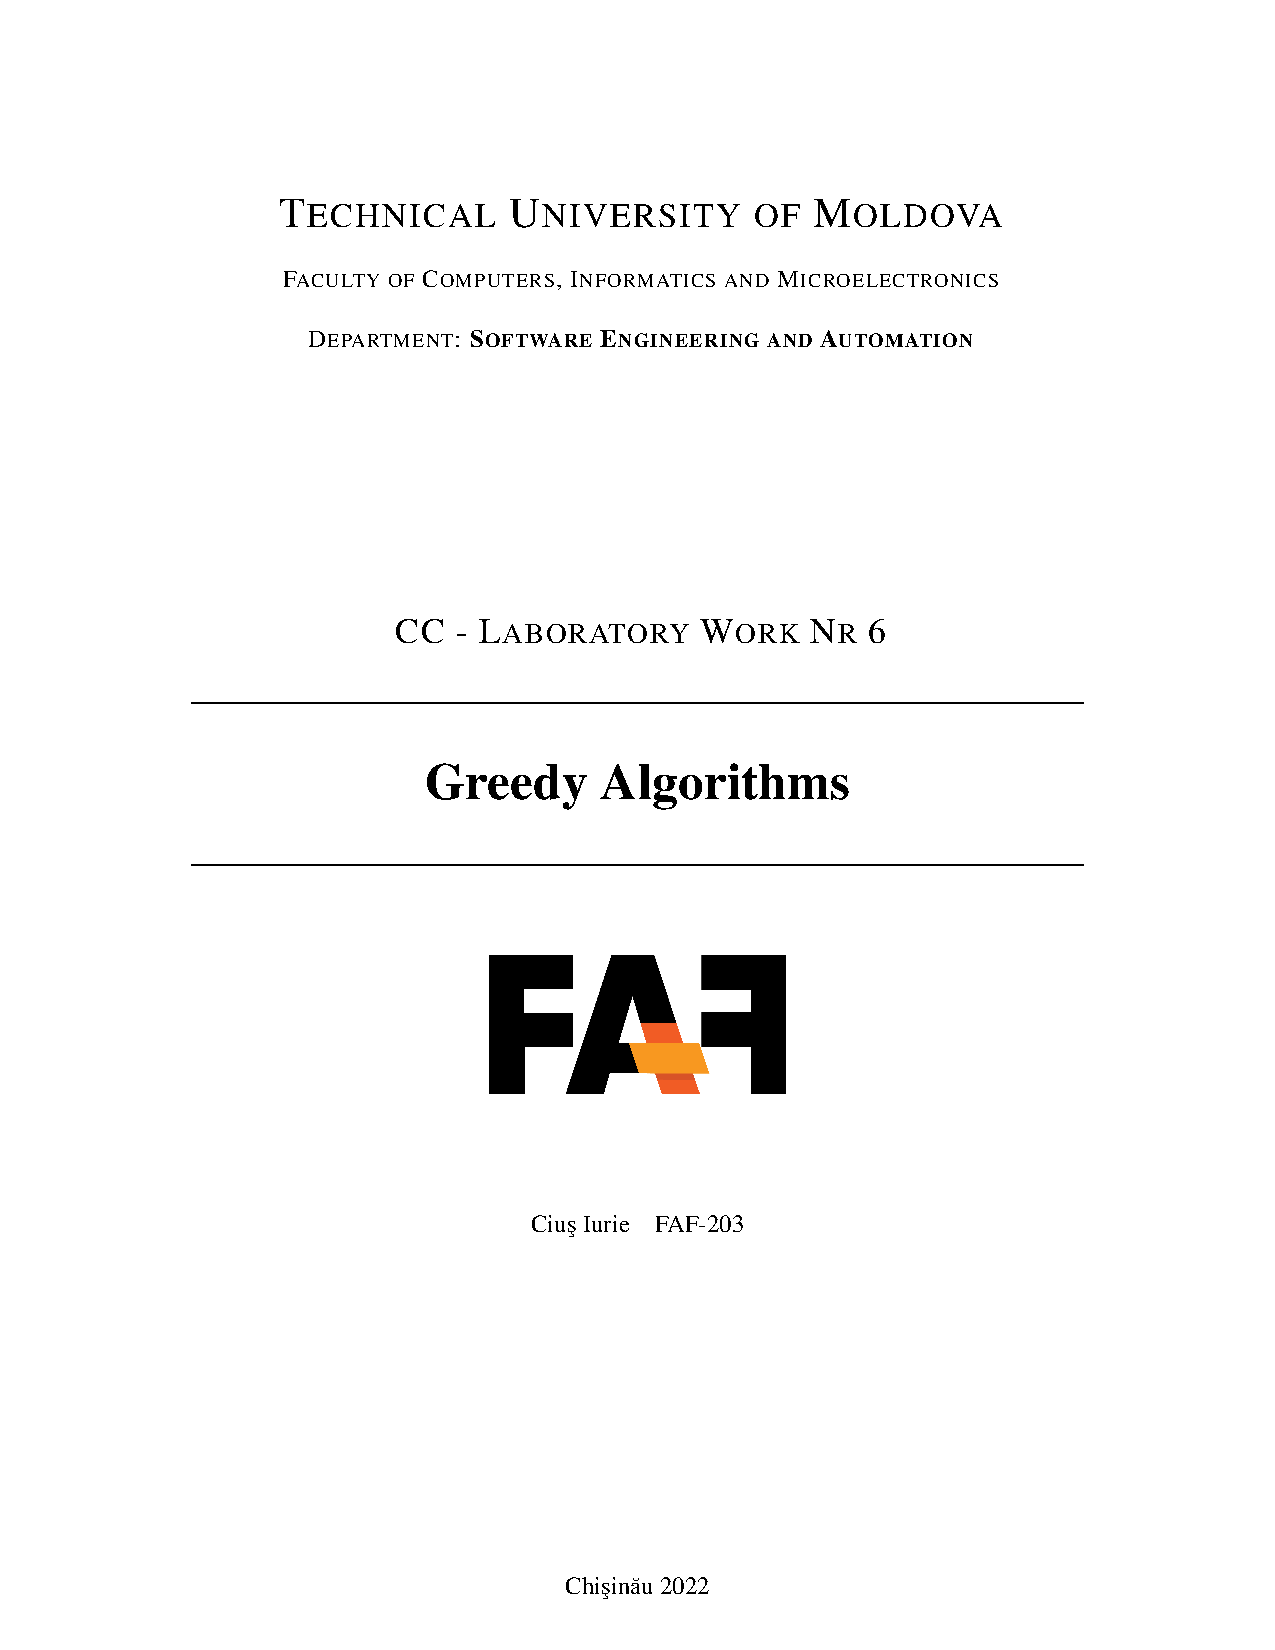
\includepdf[pages={1}]{title.pdf}
\tableofcontents
\newpage

\section{Algorithm Analysis}

Algorithm analysis is an important part of computational complexity theory, which provides
theoretical estimation for the required resources of an algorithm to solve a specific computational problem. Analysis of algorithms is the determination of the amount of time and space
resources required to execute it.

\subsection{Introduction}

A greedy algorithm is any algorithm that follows the problem-solving heuristic of making the locally optimal choice at each stage.  In many problems, a greedy strategy does not produce an optimal solution, but a greedy heuristic can yield locally optimal solutions that approximate a globally optimal solution in a reasonable amount of time.
For example, a greedy strategy for the travelling salesman problem (which is of high computational complexity) is the following heuristic: "At each step of the journey, visit the nearest unvisited city." This heuristic does not intend to find the best solution, but it terminates in a reasonable number of steps; finding an optimal solution to such a complex problem typically requires unreasonably many steps. In mathematical optimization, greedy algorithms optimally solve combinatorial problems having the properties of matroids and give constant-factor approximations to optimization problems with the submodular structure.

Greedy algorithms produce good solutions on some mathematical problems, but not on others. Most problems for which they work will have two properties:

\textbf{Greedy choice property}

We can make whatever choice seems best at the moment and then solve the subproblems that arise later. The choice made by a greedy algorithm may depend on choices made so far, but not on future choices or all the solutions to the subproblem. It iteratively makes one greedy choice after another, reducing each given problem into a smaller one. In other words, a greedy algorithm never reconsiders its choices. This is the main difference from dynamic programming, which is exhaustive and is guaranteed to find the solution. After every stage, dynamic programming makes decisions based on all the decisions made in the previous stage and may reconsider the previous stage's algorithmic path to the solution.

\textbf{Optimal substructure}

"A problem exhibits optimal substructure if an optimal solution to the problem contains optimal solutions to the sub-problems."

\subsection{Objectives}

\begin{itemize}
      \item To study the greedy technique of designing algorithms.
      \item
            To be implemented in a programming language algorithms
            Prim and Kruskal.
      \item To make the empirical analysis of the Kruskal and Prim algorithms.
      \item To make a report.
\end{itemize}

\subsection{Control questions:}

\begin{itemize}
      \item Describe the greedy method.
      \item When is the Kruskal algorithm applied and when is the Prim algorithm?
      \item How algorithm performance can be improved
            Right?
      \item What type of data is convenient to use when developing the program
            of a greedy algorithm?
      \item What are the advantages and disadvantages of Prim and Algorithms
            Kruskal?
\end{itemize}

\newpage

\subsection{Theoretical Notes}

The Greedy Algorithm solves problems by making choices that seem best fitting during a particular moment. The use of this algorithm often appears throughout many optimization problems. Greedy algorithms provide efficient solutions that is close to optimal under two properties: one of them being the “Greedy Choice Property” which makes locally optimal decisions based on its current situation and the second being: “Optimal Structure” which contains solutions to sub problems of an optimal solution. However, Greedy algorithms at times fail to come to a global optimal solution because they don’t exhaustively work on all of the data at once. This is an issue because making certain decisions early on in the algorithm can prevent it from finding the best overall solution later on. This being said, if a Greedy algorithm can be proven to generate the global optimum of a given problem, it becomes the method of choice because it is faster than any other optimization methods such as Dynamic Programming etc.

Greedy algorithms are simple instinctive algorithms used for optimization (either maximized or minimized) problems. This algorithm makes the best choice at every step and attempts to find the optimal way to solve the whole problem.

\textbf{Kruskal's Algorithm} is used to find the minimum spanning tree for a connected weighted graph. The main target of the algorithm is to find the subset of edges by using which we can traverse every vertex of the graph.

\textbf{Prim's Algorithm} is a greedy algorithm that is used to find the minimum spanning tree from a graph. Prim's algorithm finds the subset of edges that includes every vertex of the graph such that the sum of the weights of the edges can be minimized.

An improved \textbf{Dijkstra shortest path algorithm} might look like this. The improved algorithm introduces a
constraint function with weighted value to solve the defects of
the data structure storage, such as lots of redundancy of space
and time. The number of search nodes is reduced by ignoring
reversed nodes and the weighted value is flexibly changed to
adapt to different network complexity.

\newpage

\subsection{Description of The Algorithms}

The components that can be used in the greedy algorithm are:

\begin{itemize}
      \item \textbf{Candidate set:} A solution that is created from the set is known as a candidate set.
      \item \textbf{Selection function:} This function is used to choose the candidate or subset which can be added in the solution.
      \item \textbf{Feasibility function:} A function that is used to determine whether the candidate or subset can be used to contribute to the solution or not.
      \item \textbf{Objective function:} A function is used to assign the value to the solution or the partial solution.
      \item \textbf{Solution function:} This function is used to intimate whether the complete function has been reached or not.
\end{itemize}

\newpage

\section{Code}

\subsection{Implementation}

\subsubsection*{Prim Algorithm}
\lstinputlisting[language=Java]{script.java}


\subsubsection*{Kruskal Algorithm}
\lstinputlisting[language=Java]{kruskal.java}

\newpage

\subsection{Complexity of the Algorithms}

\subsubsection*{Prim’s Algorithm}

The time complexity of Prim's algorithm depends on the data structures used for the graph and for ordering the edges by weight, which can be done using a priority queue. The following table shows the typical choices:

\begin{center}
      \begin{tabular}{|c|c|}
            \hline
            Minimum edge weight data structure & Time complexity (total)                       \\
            \hline
            adjacency matrix, searching        & $O(\|V\|^2)$                                  \\
            \hline
            binary heap and adjacency list     & $O((\|V\|+\|E\|)log\|V\|) = O(\|E\|log\|V\|)$ \\
            \hline
            Fibonacci heap and adjacency list  & $O(\|E\|+\|V\|log\|V\|)$                      \\
            \hline
      \end{tabular}
\end{center}

\subsubsection*{Kruskal's Algorithm}

Kruskal’s Algorithm builds the spanning tree by adding edges one by one into a growing spanning tree. Kruskal's algorithm follows greedy approach as in each iteration it finds an edge which has least weight and add it to the growing spanning tree.

This could be done using DFS which starts from the first vertex, then check if the second vertex is visited or not. But DFS will make time complexity large as it has an order of \textbf{O(V+E)} where V is the number of vertices, E is the number of edges.

\subsection{Graphs}

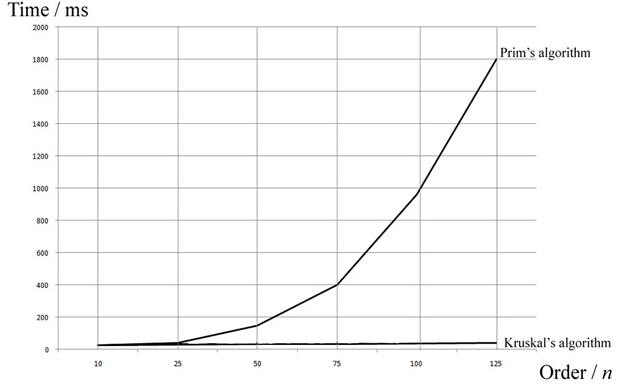
\includegraphics[width=14cm]{img1.png}

\section{Conclusion}

To conclude, the current piece of work represents my personal implementation of
2 greedy algorithms - Prim's and Kruskal. The programming language I chose is
Java. The results show the time performance in seconds based on the N nodes.
As you can see in the \textit{Figure 1}, the Kruskal algorithms performed the best with
a complexity of O(0), while the last one - $O(n^2)$.

\subsection{References}

\begin{itemize}
      \item https://github.com/IuraCPersonal
\end{itemize}


\end{document}